\addcontentsline{toc}{chapter}{Biographical Sketch}
\chapter*{Biographical Sketch}
\noindent
\begin{minipage}{0.3\textwidth}
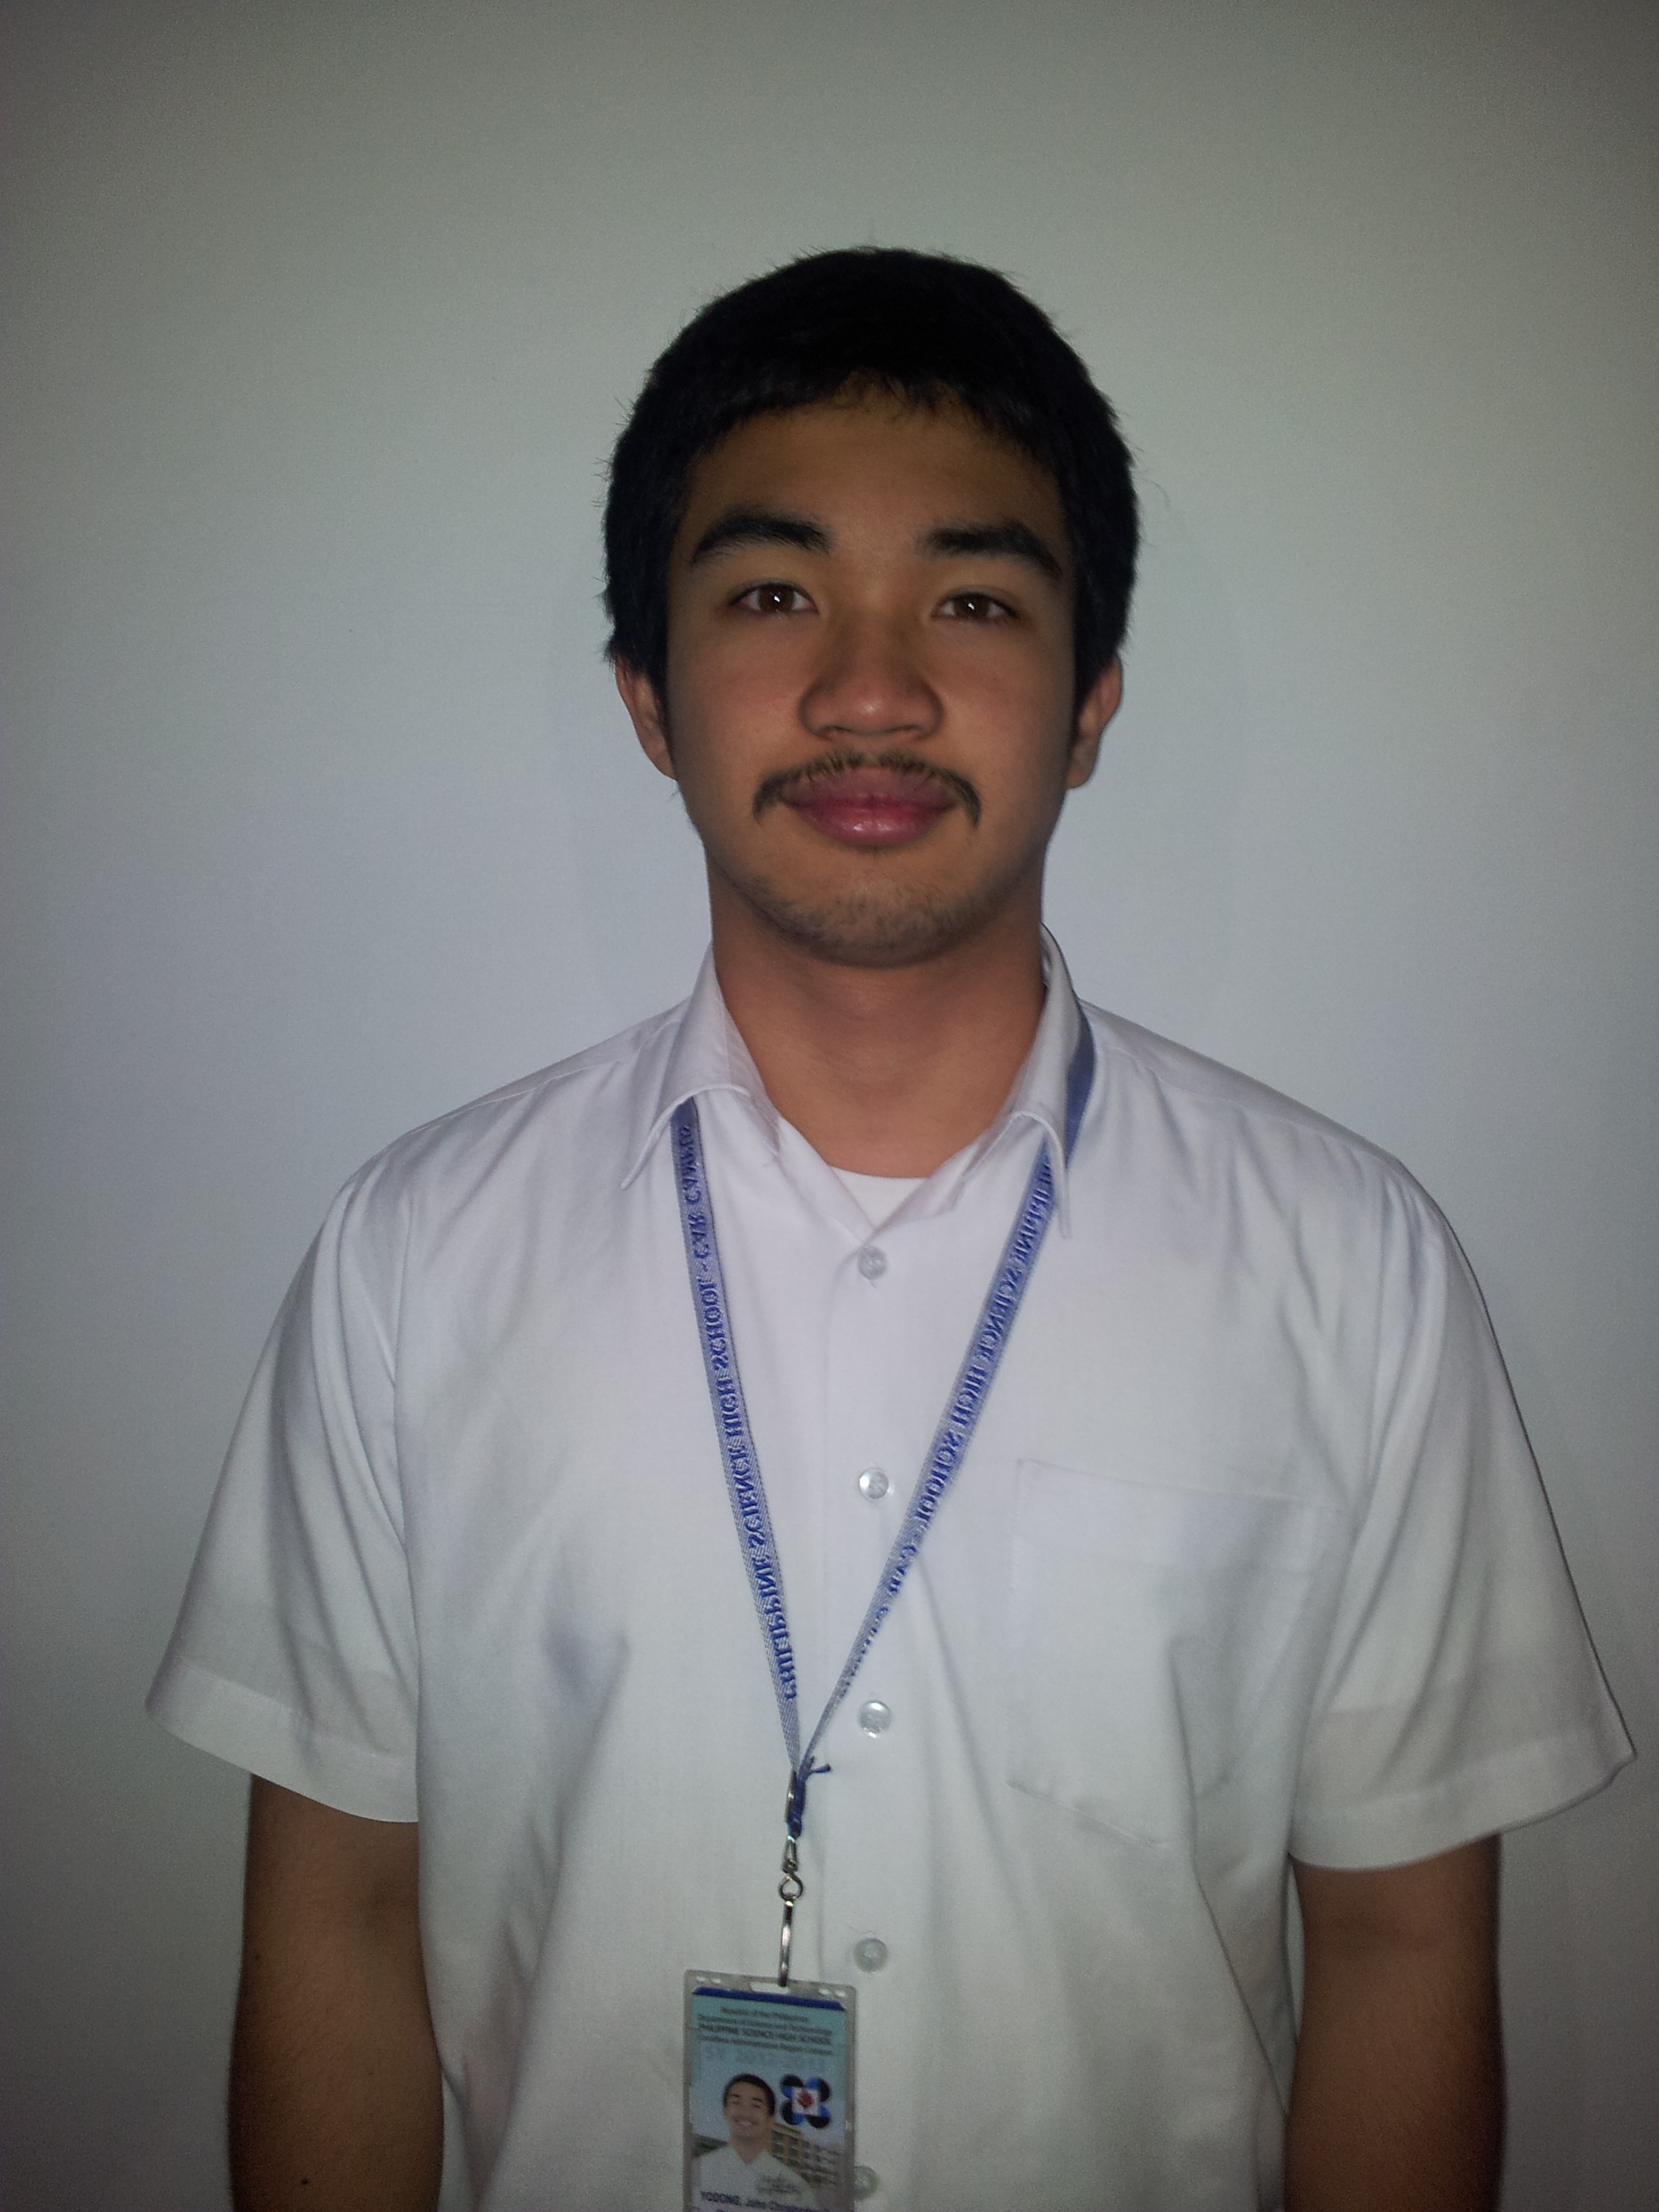
\includegraphics[width=0.8\linewidth]{2013-03-04-17-00-28}
\end{minipage}\hfill
\begin{minipage}{0.68\textwidth}
\textbf{John Christopher C. Yodong}, born on October 06, 1996, is a graduate of SPED Center Elementary School and is currently a fourth year student in PSHS-CAR campus. He is a citizen of the Republic of the Philippines and he is a resident of Baguio City. He is a consistent learner and he is able to perform well in school.  He, along with Sheanne Eric P. Cabantac and Mikhail Antoni A. Osbucan, is one of the proponents of the research on the series analysis of rainfall in Baguio City. 
\end{minipage}

\vfill

\noindent
\begin{minipage}{0.68\textwidth}
\textbf{Mikhail Antoni Azul Osbucan} is currently studying at Philippine Science High School. He is currently a member of  the section IV-Photon. He was born on the 30th day of March on 1997 in Baguio City. He is the first child of Ma. Lourdes Osbucan and Rommel Paolo Osbucan. He is of Igorot, Bisayan, and Tagalog decent. He likes to play basketball a lot and he also watches NBA a lot. He is a big fan of alternative music. He is also a big fan of action and suspense movies. When he grows older, he wants to become either a successful pilot or a successful cardiologist. He also believes in the saying that “Hardwork beats talent when talent fails to work hard.” 
\end{minipage}\hfill
\begin{minipage}{0.3\textwidth}\raggedleft
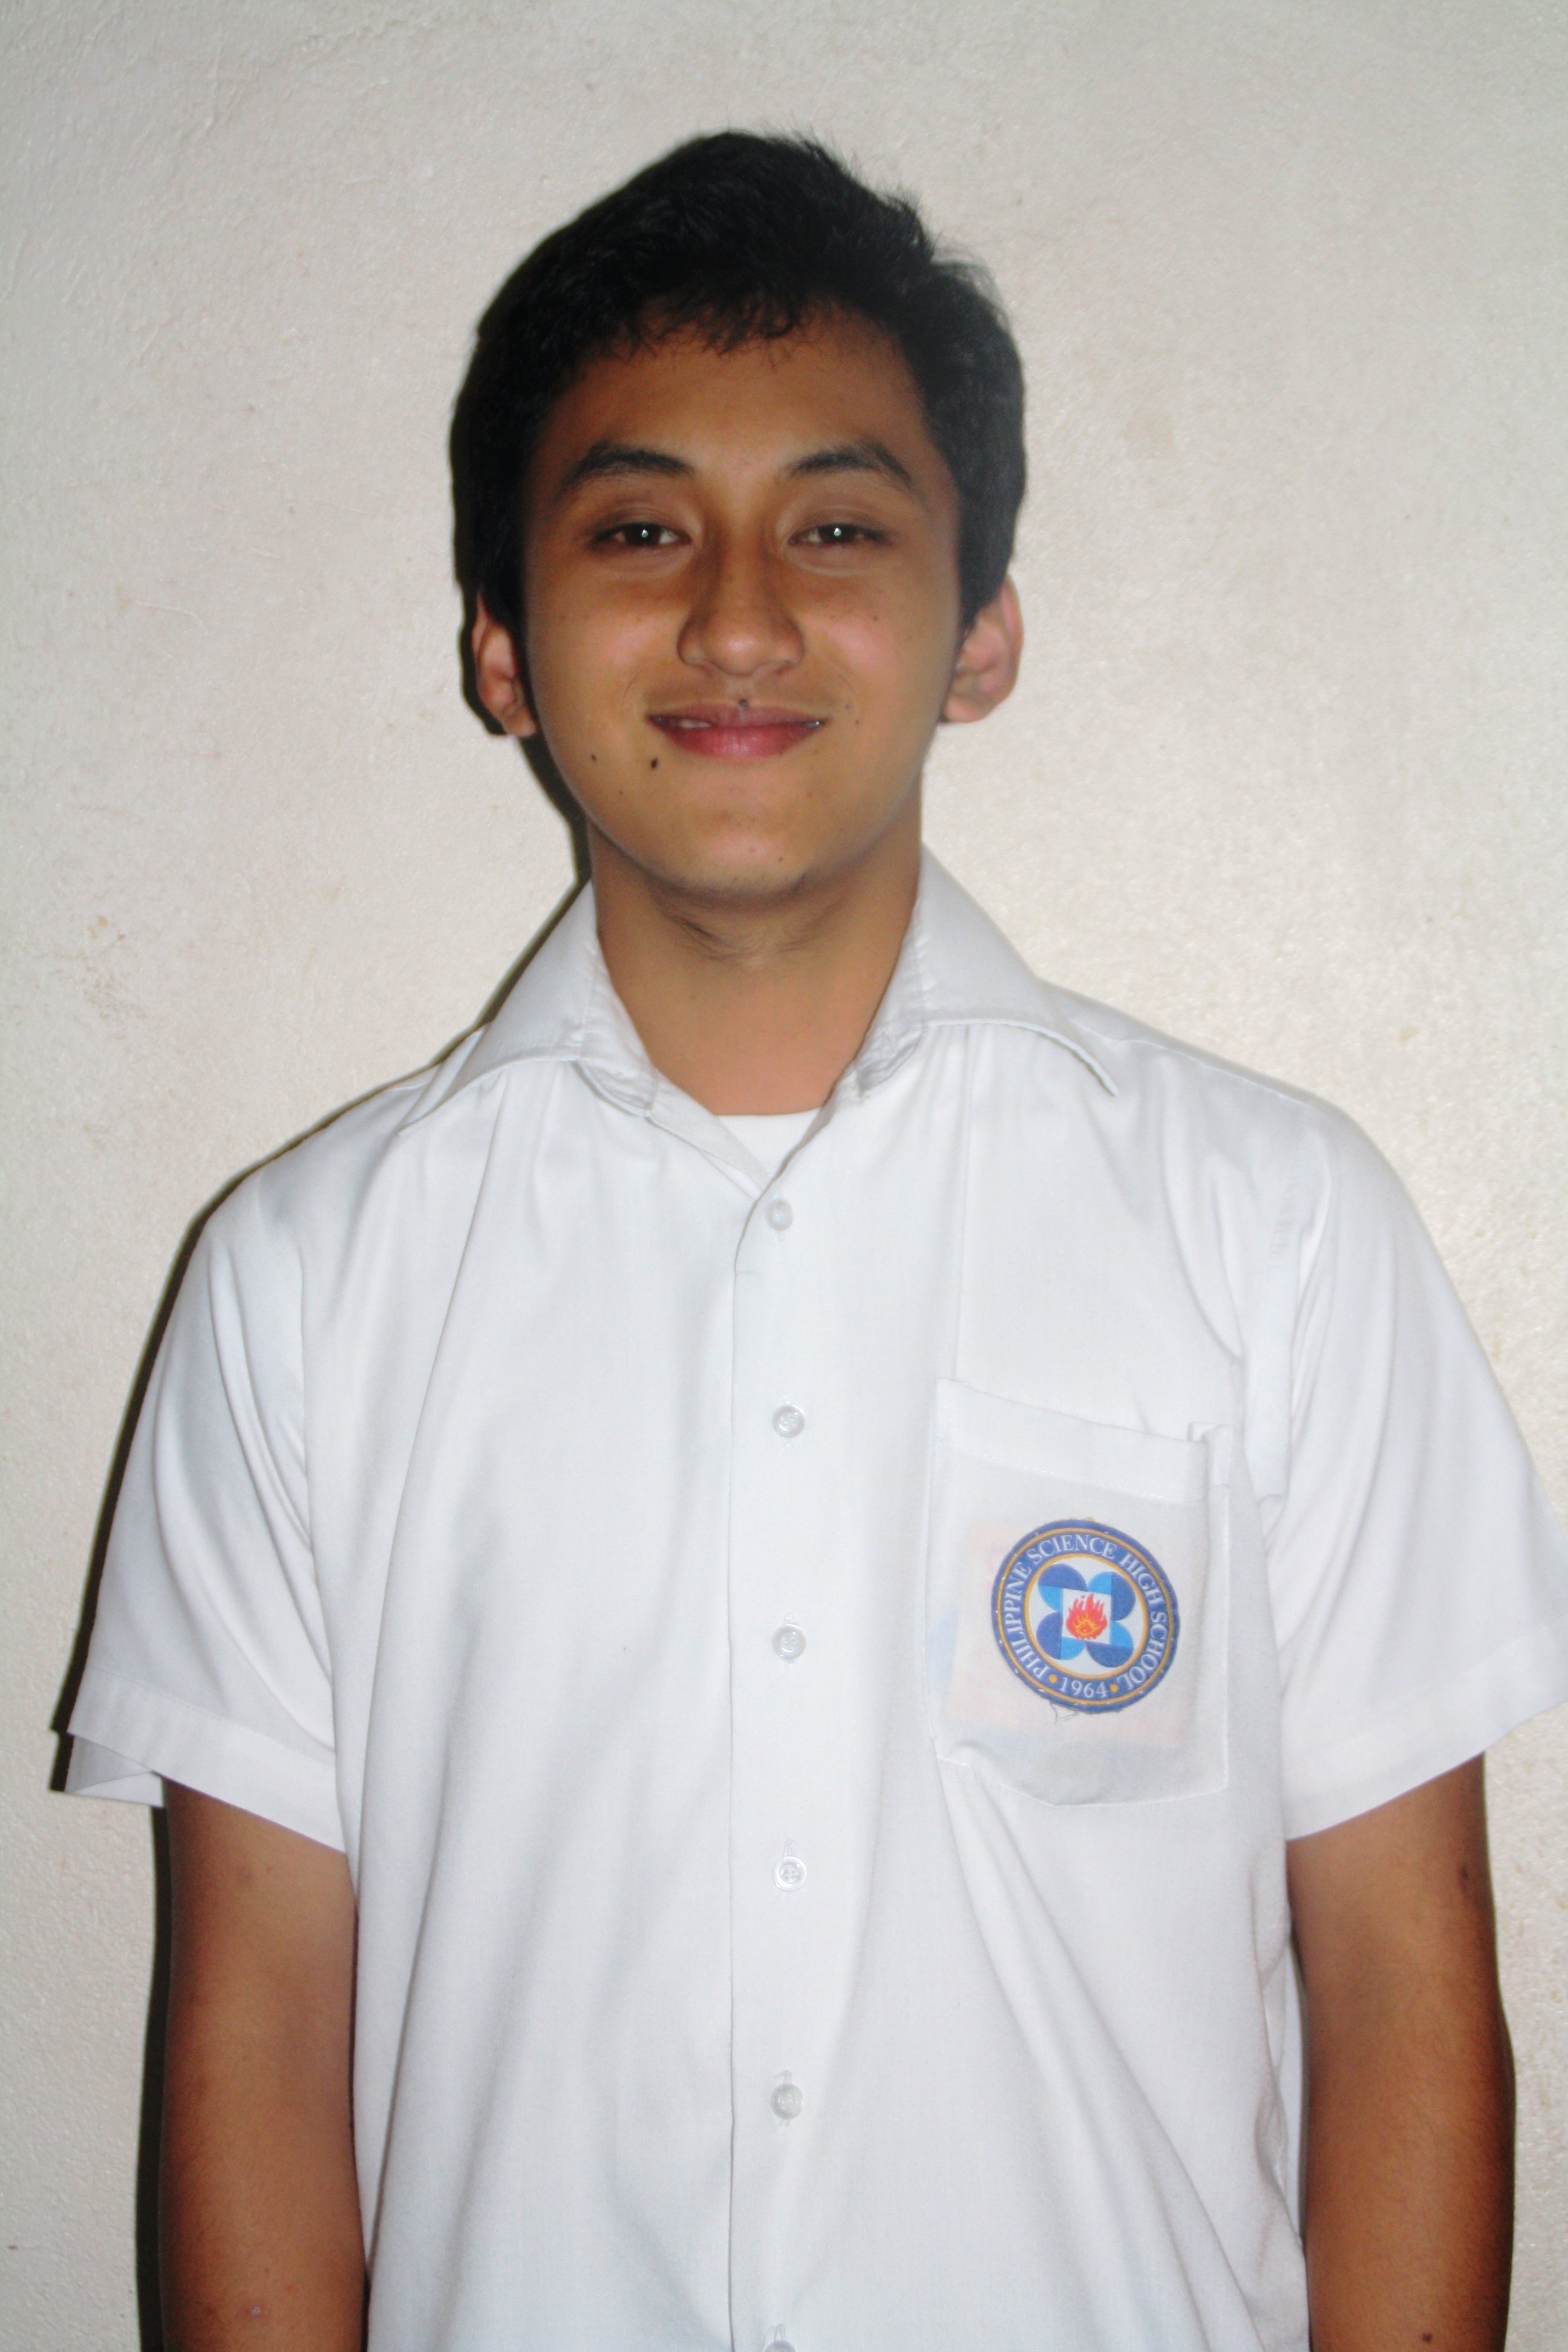
\includegraphics[width=0.8\textwidth]{IMG_5287}
\end{minipage}

\vfill

\noindent
\begin{minipage}{0.3\textwidth}
\includegraphics[width=0.8\textwidth, keepaspectratio]{IMG_5656}
\end{minipage}\hfill
\begin{minipage}{0.68\textwidth}
\textbf{Sheanne Eric P. Cabantac} is a Filipino citizen, born and raised in Baguio City on January 14,1997. He completed his primary education in Star Educational School in La Trinidad and graduated as an academic achiever. He then pursued his elementary education at SPED Center Baguio City, before getting to Philippine Science High School CAR Campus. He is a son to Eduardo R. Cabantac and Sheryl Anne P. Cabantac, and an older brother to three siblings.
\end{minipage}